\chapter{Aufbau und Struktur M1 Modell} \label{M1Modell}
Beim M1 Modell handelt es sich um die direkte Darstellung der zu generierenden
Views für die Webanwendung. Dieses Modell wird direkt durch den Generator,
siehe Abschnitt \ref{Generator}, umgesetzt und um alle zusätzlichen Dateien
erweitert, die für die Ziel-Architektur notwendig sind. Das Ziel, in dieser
Ausarbeit, lag vor allem darin die Ziel-Architektur mit möglichst wenig Aufwand
für den Entwickler zu generieren, somit ist das M1 Modell nicht als vollständige
Abbildung des Projektes zu verstehen. Das Erzeugen des Modells sollte
übersichtlich gestaltet werden, um einerseits den Programieraufwand zu
minimieren und anderseits die Fehlerquote zu verringern.

In dieser Arbeit, soll der Generator aus dem M1 Modell, die im Abschnitt
\ref{AufBZielArchitektur} beschriebene mögliche Grundstruktur für ein GWT
Projekt erzeugt werden. Dieses kann durch kleine Änderungen lauffähig gemacht
werden. Das M1 Modell ist so angedacht, dass alle Seiten, der Webanwendung, als
eine eigenständige View dargestellt werden. Des Weiteren können
einfache Elemente, wie beispielsweise Label und Textfelder den Views hinzugefügt
werden. Zudem ist es möglich die Navigation zwischen den Seiten, beispielsweise
mit Hilfe eines Menus, in das Modell mit einzubringen. 

Durch die Verwendung eines Profils sind in dem M1 Modell keine Assoziationen
zu sehen. Die Navigation wird ausschließlich über die Properties in den
Navigations Elementen erstellt, in dieser Arbeit werden diese Elemente mit dem
Stereotyp \textit{ViewNavigationObject} gekennzeichnet. Der einfache
Grundaufbau des M1 Modells, sorgt für eine leichtere Modellierung, erschwert
allerdings das Erkennen der Navigation.

\section{M1 Modellaufbau}
Wenn ein neues Projekt angelegt wird, muss in den Properties des M1 Modells
neben der Angabe des Profils ein Name definiert werden. Dieser Name stellt
später den Hauptpaketnamen des GWT Projektes dar und legt somit den Grundstein
für die Paketstruktur (vgl. Abbildung \ref{Fig:mainpackage}).

\begin{figure}[htbp]
\begin{center}
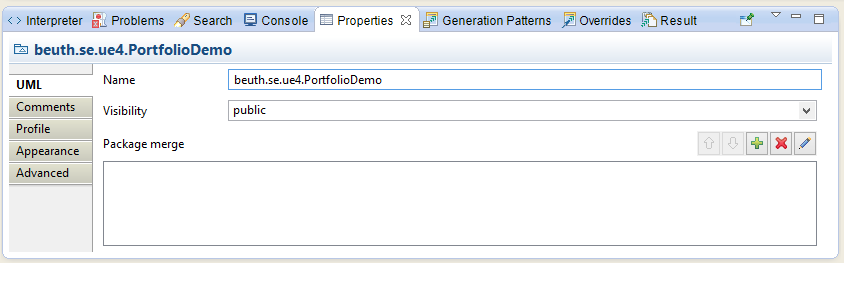
\includegraphics[width=0.8\textwidth]{./img/ProjectPackage.png}
\caption{Name des Modells und gleichzeitig Hauptpaket des
GWT Projekts}\label{Fig:mainpackage}
\end{center}
\end{figure}

\newpage
\section{Klassenaufbau}
Die grundlegendsten Elemente in dem Modell sind \textit{ViewImpl} Klassen. Ein
Beispiel dafür ist in Abbildung \ref{Fig:viewimpl} zu sehen. Für jede dieser
Klassen, werden durch den Generators, alle notwendigen Dateien
erzeugt die für den späteren Aufruf, der Seite, notwendig sind.

\begin{figure}[htbp]
\begin{center}
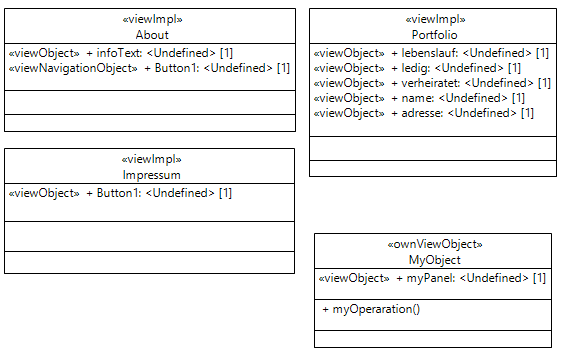
\includegraphics[width=1.0\textwidth]{./img/GWT-Model-Views-alg.png}
\caption{\textit{ViewImpl} Klassen zur Erzeugung von Seiten
für den Webauftritt.}\label{Fig:viewimpl}
\end{center}
\end{figure}

Des Weiteren ist in der Abbildung \ref{Fig:viewimpl} ein Beispiel für ein
\textit{OwnViewObject} zu sehen. Diese sind für komplexere oder mehrfach
verwendete UI Strukturen gedacht und werden vom Generator als eigenständige
Klasse generiert.

Die Ziel-Architektur bietet, durch Verwendung des MVP Pattern, eine einfache
Möglichkeit View Implementierungen auszutauschen. Um dieses Verfahren in
jedem Fall für den Entwickler nutzbar zu machen, wurde sich dazu entschlossen,
neben der Generierung von View Implementierungen, eine zusätzliche Methode
einzubauen. Diese Methode bietet die Möglichkeit beliebig viele alternativ
Seiten für ein View Interface zu erzeugen (vgl. Abbildung
\ref{Fig:viewInterface}). Die Möglichkeit der einfachen Austauschbarkeit von
Views, wurde bei GWT unter anderem für Testzwecke angedacht.

\begin{figure}[htbp]
\begin{center}
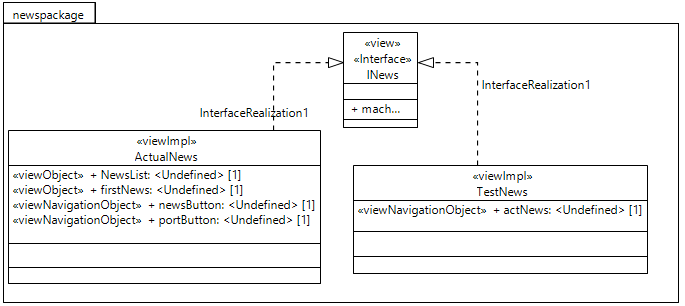
\includegraphics[width=1.0\textwidth]{./img/GWT-Model-Views-interface.png}
\caption{Ein Beispiel für die Verwendung der \texttt{ViewInterface}-Klassen
um mit Hilfe einer Vielzahl von \texttt{ViewImpl}-Klassen
eine austauschbare Ansicht zu erzeugen.}\label{Fig:viewInterface}
\end{center}
\end{figure} 

Bei dem, in Abbildung \ref{Fig:viewInterface}, gezeigtem M1 Modell Ausschnitt
wird die komplette Klassenstruktur nicht zweimal erzeugt, anders als im
allgemeinem Fall (siehe Abbildung \ref{Fig:viewimpl}). Die
\texttt{'Name'Activity.java}, \texttt{'Name'Place.java} und \\
\texttt{'Name'View.java} Klassen werden hierbei nur einmal für das Interface
und die \texttt{'Name'ViewImpl.java} und \texttt{'Name'ViewImpl.ui.xml}
Dateien für jede realisierende \texttt{ViewImpl}-Klasse generiert. 

Darüber hinaus ist in Abbildung \ref{Fig:viewInterface} zu sehen, dass es
möglich ist, Klassen zu Paketen zuzuordnen. Auf diese Weise wird es
ermöglicht die zu generierenden Dateien zu gruppieren. 

\newpage
Das letzte in den Modellen genutzte Klassenkonstrukt, sind die sogenannten
\textit{PermanentViewImpl}-Klassen. Diese sind dazu gedacht, um zum Beispiel
Menus zu erzeugen. Diese haben die Eigenschaft das sie auf allen Webseiten zur
Verfügung stehen und bei der Generierung nicht mehrfach in die normalen Views
eingebunden werden sollen.

\begin{figure}[htbp]
\begin{center}
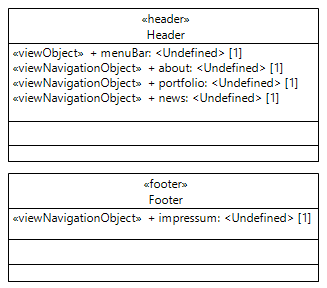
\includegraphics[width=0.55\textwidth]{./img/Header_Footer.png}
\caption{\textit{PermanentViewImpl}-Klassen am Beispiel
eines Headers, mit Menu, und eines Footers.}\label{Fig:headerFooter}
\end{center}
\end{figure} 

\section{Seitenaufbau}
Je nach Art der View muss zuerst definiert werden, um was für einen Typ von
View es sich handelt. In Abbildung \ref{Fig:SideProp} ist ein Beispiel dafür
zu sehen, welches eine \textit{ViewImpl} und ein \textit{Header} zeigt, eine
spezialisierte Form der \textit{PermanentViewImpl}. Wichtig ist hier
die \texttt{concreteBinding}-Eigenschaft. An dieser Stelle kann bei Verwendung
eines separaten Interfaces festgelegt werden, welche konkrete Implementierung
dargestellt werden soll. Um keine Laufzeitfehler zu erzeugen muss zu jeder View
exakt eine \textit{ViewImpl} angegeben werden. Diese Einstellung kann später im
Quellecode geändert werden.

\newpage
\begin{figure}[htbp]
\begin{center}
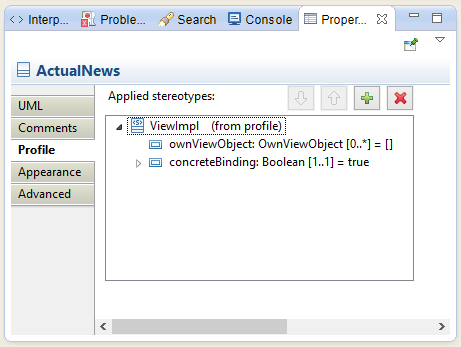
\includegraphics[width=0.8\textwidth]{./img/Prop-ViewImp.png}
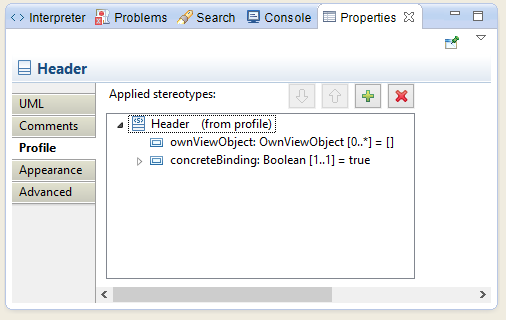
\includegraphics[width=0.8\textwidth]{./img/Prop-Header.png}
\caption{Klassen mit definierten Stereotypen, oben
eine \textit{ViewImpl} und unten ein \textit{Header}}\label{Fig:SideProp}
\end{center}
\end{figure} 

Um diese Views mit Inhalten zu befüllen, können \textit{ViewObject}s und 
\textit{ViewNavigationObject}s als Attribute hinzugefügt werden.

\newpage
Bei \textit{ViewObject}-Elementen können die in Abbildung \ref{Fig:ViewProp}
dargestellten Eigenschaften verändert werden.

\begin{figure}[htbp]
\begin{center}
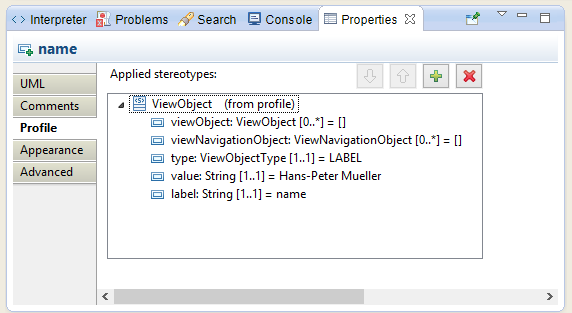
\includegraphics[width=0.8\textwidth]{./img/Prop-ViewObjects.png}
\caption{Eigenschaften eines \textit{ViewObject}-Elementes }\label{Fig:ViewProp}
\end{center}
\end{figure} 

Bei \textit{ViewNavigationObject}-Elementen können die in Abbildung
\ref{Fig:ViewNavProp} dargestellten Eigenschaften verändert werden. Hier ist
vor allem die letzte Eigenschaft \texttt{goToView} zu beachten, welche angibt
wohin dieses navigieren soll.

\begin{figure}[htbp]
\begin{center}
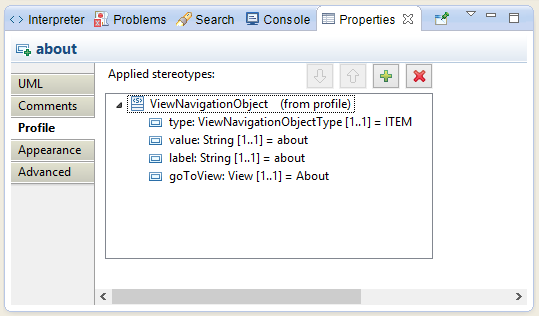
\includegraphics[width=0.8\textwidth]{./img/Prop-ViewNavigationObjects.png}
\caption{Eigenschaften eines \textit{ViewNavigationObject}-Elementes
}\label{Fig:ViewNavProp}
\end{center}
\end{figure}
